% Main entry for the IEEE Aerospace Conference 2026 version of the
% effective-wrench residual modeling paper.

\documentclass[twocolumn,letterpaper]{IEEEAerospaceCLS}

% Packages and general settings for the AeroConf version of the paper.

\usepackage{graphicx}
\usepackage{xcolor}
\usepackage{amsmath,amssymb}
\usepackage{booktabs}
\usepackage{cite}
\usepackage[colorlinks=true, urlcolor=blue, linkcolor=black, citecolor=black]{hyperref}

% Common macros used across sections.

\newcommand{\Fxbar}{\bar{F}_x}
\newcommand{\Fzbar}{\bar{F}_z}
\newcommand{\Pinbar}{\bar{P}_{in}}
\newcommand{\etabar}{\bar{\eta}}

\newcommand{\deltads}{\delta}
\newcommand{\Tperiod}{T}
\newcommand{\Uinf}{U}
\newcommand{\feff}{f_{\mathrm{eff}}}
\newcommand{\needinfo}[1]{\textcolor{red}{#1}}


\pdfminorversion=7

\title{Theory-Guided Neural Residual Modeling of Real-Flight Effective Wrench for Flapping-Wing Simulation}

\author{%
TODO Author Name\\
TODO Affiliation\\
TODO Postal Address\\
TODO Email
\thanks{\footnotesize 979-8-3315-7360-7/26/$\$31.00$ \copyright2026 IEEE}
}

\begin{document}

\maketitle

\thispagestyle{plain}
\pagestyle{plain}

% !TeX root = ../main.tex
\begin{abstract}
Accurate force and moment models are needed for flapping-wing simulation, control design, and flight-log interpretation, but physics-based models often leave systematic errors when applied to outdoor flight of a complete vehicle. This letter studies real-flight effective-wrench modeling for a bird-scale flapping-wing vehicle. We derive six-component body-frame effective wrench labels from onboard flight logs and align them with a DeLaurier-style simulator prior. Instead of replacing the prior with a black-box model, we formulate a theory-guided residual problem in which a causal neural model predicts the remaining discrepancy between the calibrated simulator prior and the log-derived effective wrench. On held-out whole-log tests, the calibrated prior has an overall RMSE of $5.97$, while a residual Transformer reduces the combined prediction error to $0.85$. In date-stratified five-fold whole-log evaluation, the reduction is stable, from $5.883\pm0.040$ to $0.827\pm0.027$ RMSE. Residual analysis shows that the remaining DeLaurier mismatch is not random: the main force-channel residuals contain repeatable wingbeat-phase, frequency, and flight-condition structure, and the neural residual removes most of this structured discrepancy. These results support theory-guided neural residual modeling as a practical route for bringing real-flight effects into flapping-wing simulation.
\end{abstract}


\tableofcontents

% !TeX root = ../main.tex
\section{Introduction}
\label{sec:introduction}

Future flapping-wing aerial vehicles are expected to do more than maintain stable flight. A practical vehicle may need to regulate flight while also using perception, interacting with targets, grasping or perching, and making task-level decisions in outdoor environments. This broader autonomy goal makes reinforcement learning attractive, because flight states, visual observations, contact or interaction cues, and task rewards can be handled within a single training framework~\cite{kober2013rlsurvey}. The same breadth also makes direct hardware training difficult. Real flight tests expose the vehicle to actuator limits, wind, impact, and recovery failures, and broad generalization would require data from many successful and unsuccessful operating conditions.

Real flight logs are therefore valuable but not sufficient by themselves. They contain the actual vehicle response, actuator behavior, sensing effects, and outdoor disturbances, yet they usually cover only the state distribution that has already been flown. For a bird-scale flapping-wing platform, collecting enough logs to cover aggressive maneuvers, rare disturbances, failure cases, and wide operating envelopes can be impractical. This limitation pushes future learning, controller design, trajectory replay, and task-level evaluation toward simulation. A useful simulator, however, must contain a model of the flapping-wing dynamics that is both accurate enough to be meaningful and fast enough for repeated rollouts.

For flapping-wing vehicles, the main modeling bottleneck is aerodynamics. The vehicle generates forces and moments through periodic wing motion, wing flexibility, tail and body aerodynamics, and coupled motion between the fuselage and wings. High-fidelity computational fluid dynamics can resolve more of this flow physics, but it is too slow for large-scale controller training or repeated evaluation. Vortex-based and reduced-order approaches provide intermediate fidelity. Empirical and semi-empirical formulations sacrifice some physical detail for speed, but their structure makes them practical simulator priors. In this paper, DeLaurier's flapping-wing aerodynamic formulation~\cite{delaurier1993} is used as such a prior.

Speed alone does not make an empirical prior flight-realistic. A nominal aerodynamic calculation cannot fully capture airframe-specific geometry, wing deformation, actuator timing, tail effectiveness, body--wing interaction, sensor alignment, and state-estimation errors. Outdoor flight also adds wind and airframe-condition variation. Domain randomization and dynamics randomization can improve robustness when policies are transferred from simulation to hardware~\cite{tobin2017domainrandomization,peng2018dynamicsrandomization}, but randomization is most useful when the simulator prior and its systematic errors are understood. If a repeatable part of the gap is aerodynamic, the first engineering problem is to diagnose where the simulator prior differs from real flight and whether that residual can be predicted from onboard measurements.

Flight data have long been used to make flapping-wing models useful beyond idealized aerodynamic analysis. Early DelFly studies reconstructed aerodynamic forces and moments from motion-capture flight tests and identified simple linear or time-varying models, often at a flap-averaged or low-order modeling level~\cite{caetano_linear_2013,armanini_time-varying_2016}. Related grey-box and onboard-sensor-based methods have been reported for tailless flapping-wing micro air vehicles and longitudinal stability analysis~\cite{nijboer_longitudinal_2020,aurecianus_longitudinal_2022}. At larger scales, flight-data studies of ornithopters have examined force estimation, trim behavior, and periodic state variation in forward flight~\cite{aminietal2020largescale}. More recent avian-inspired platforms show that real flight data can expose flapping-period structure: phase-functioned neural models have predicted equivalent aerodynamic forces and moments from flight data~\cite{zhao2025phase}, and learned periodic corrections from onboard inertial and GNSS data have improved state estimation for a $1.7~\mathrm{m}$ wingspan vehicle~\cite{qian_learning_2026}.

Controlled aerodynamic datasets provide a complementary route to data-driven flapping-wing models. Neural models have been used to predict unsteady flapping-airfoil loads~\cite{kurtulus_ability_2009}, transient aerodynamic properties of flapping-wing systems~\cite{lan_neural_2022}, and robust reduced models for hovering flapping wings~\cite{calado_robust_2023}. Recent surrogate models also predict time-history lift, thrust, and moment curves for optimization using computational or experimental datasets~\cite{wang_time-history_2024,corban_discovering_2023,chen_data-driven_2026}. These studies demonstrate the value of data-driven aerodynamic modeling, but many rely on prescribed kinematics, wind-tunnel measurements, computational data, or bench-top experiments. Learning methods have also improved flapping-wing control, estimation, and simulation~\cite{he_adaptive_2017,qian_neural_2023,qian_learning_2023,fei_flappy_2019}. The remaining need for simulation is to connect a fast, structured aerodynamic prior to instantaneous six-axis effective force and moment labels reconstructed from outdoor flight logs of the complete vehicle.

Our platform provides the measurements needed for that connection. The vehicle flies with a PX4-based fixed-wing stack~\cite{meier2015px4} while recording synchronized state estimates, airdata, actuator commands, flapping phase, and flapping frequency. These logs allow the body-frame effective wrench required to explain the measured rigid-body motion to be reconstructed and compared directly with the wrench predicted by a DeLaurier-style simulator model. The comparison turns real flight data into a diagnostic for the aerodynamic component of the simulator gap.

This paper presents a real-flight effective-wrench residual modeling pipeline for a bird-scale flapping-wing vehicle. The paper does not train a reinforcement-learning controller. Instead, it develops one engineering step toward real-flight-corrected simulation for future learning and control. In this work, body-frame six-axis effective wrench labels are reconstructed from outdoor flight logs, aligned with a DeLaurier-style aerodynamic simulator prior, and used to calibrate that prior using training logs only. A causal neural residual model then predicts the remaining discrepancy from onboard-measurable variables. Finally, the residual is analyzed by wingbeat phase, flapping frequency, and flight condition to determine whether the simulator mismatch is structured rather than random. The main contributions are:
\begin{enumerate}
  \item We construct real-flight six-axis effective force and moment labels from outdoor flight logs of a bird-scale flapping-wing vehicle and align them with a DeLaurier-style aerodynamic simulator prior to define an effective-wrench residual modeling problem.
  \item We combine a calibrated aerodynamic prior with a causal neural residual estimator that predicts the remaining simulator-to-flight discrepancy from onboard measurements. The resulting hybrid model is evaluated on held-out logs and date-stratified whole-log cross-validation.
  \item We use phase-binned, condition-binned, and frequency-domain diagnostics to interpret the learned residual as an engineering diagnostic for simulator mismatch. The results show that the calibrated aerodynamic prior leaves repeatable wingbeat-synchronous and flight-condition-dependent force residuals, and that the neural residual estimator removes much of this structured discrepancy.
\end{enumerate}

The remainder of the paper is organized as follows. Section~\ref{sec:dataset} describes the flight platform, logging setup, and effective-wrench reconstruction. Section~\ref{sec:method} presents the calibrated aerodynamic prior and causal residual model. Section~\ref{sec:evaluation} defines the evaluation protocol, and Section~\ref{sec:results} reports prediction performance and residual-structure analysis.

% !TeX root = ../main.tex
\section{Real-Flight Effective-Wrench Dataset}
\label{sec:dataset}

\subsection{Flight Platform and Onboard Logging}
\label{subsec:platform_logging}

The dataset was collected on a bird-scale flapping-wing vehicle designed for outdoor autonomous forward flight. Table~\ref{tab:platform_params} summarizes the platform, sensing, and logging quantities that are used later for effective-wrench reconstruction and residual modeling, and Fig.~\ref{fig:platform_dataset} shows the vehicle during flight. The vehicle mass and geometry set the scale of the reconstructed force and moment labels, while the logging configuration determines which state, actuation, airdata, and wingbeat variables are available to the causal model.

\begin{table}[t]
\caption{Platform and onboard logging summary for the flapping-wing vehicle.}
\label{tab:platform_params}
\centering
\resizebox{\columnwidth}{!}{%
\begin{tabular}{@{}ll@{}}
\toprule
Item & Value or role \\
\midrule
Nominal takeoff mass & $\approx 0.95~\mathrm{kg}$; three-point weighing value \needinfo{TBD} \\
Wingspan & $1.6~\mathrm{m}$ \\
Flight speed range & $4$--$10~\mathrm{m/s}$ \\
Maximum flapping frequency & $6.8~\mathrm{Hz}$ \\
Flight controller & Pixhawk 6C Mini running PX4 fixed-wing stack \\
Primary lift/propulsion & Single main flapping mechanism \\
Tail effectors & Left/right horizontal tails and vertical tail \\
Airspeed sensing & Pitot-static probe with MS4525DO pressure sensor \\
Position sensing & RTK-capable GNSS absolute positioning \\
Wingbeat sensing & AS5600 encoder at $100~\mathrm{Hz}$ and Hall-indexed phase path \\
CG measurement & Plumb-line suspension; $\mathbf{r}_{\mathrm{CG}}$ \needinfo{TBD} \\
Inertia measurement & Bifilar-pendulum measurement; $\mathbf{I}_{B,\mathrm{CG}}$ \needinfo{TBD} \\
IMU-to-CG survey & Mechanical survey used for reference-point alignment; $\mathbf{r}_{\mathrm{IMU}/\mathrm{CG}}^{B}$ \needinfo{TBD} \\
Actuator logging & \texttt{actuator\_motors} and \texttt{actuator\_servos}, binned to $100~\mathrm{Hz}$ \\
Low-rate context & Airdata, wind, GPS, status, and allocator topics with freshness masks \\
Canonical sample rate & $100~\mathrm{Hz}$ after offline resampling \\
\bottomrule
\end{tabular}%
}
\end{table}

\begin{figure}[t]
  \centering
  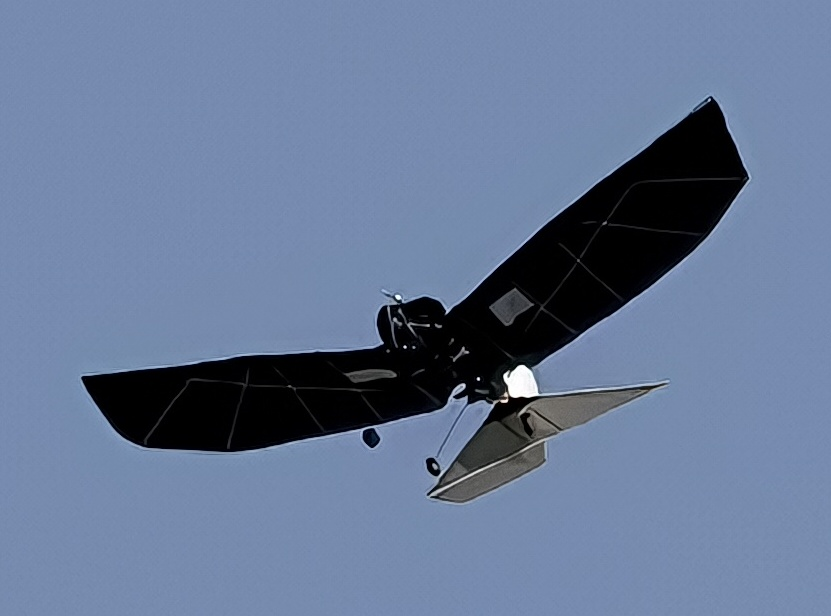
\includegraphics[width=0.98\columnwidth]{imgs/flying_img.jpg}
  \caption{Bird-scale flapping-wing vehicle during outdoor flight.}
  \label{fig:platform_dataset}
\end{figure}

The airframe uses a single motor-driven flapping mechanism to drive the two main wings and generate the dominant lift and propulsive force during forward flight. Attitude control is provided by three movable tail surfaces: the left and right horizontal tails act as elevon-like pitch and roll effectors, and the vertical tail provides yaw control. This actuation layout is important for the dataset definition because the reconstructed labels are not isolated wing loads. They are the net non-gravitational body-frame wrench that explains the measured rigid-body motion, including wing, tail, body, mechanism, and disturbance effects that are not separable from onboard logs alone.

The rigid-body quantities used in the wrench reconstruction are measured independently from the training logs. The vehicle mass is obtained with a three-point weighing setup, the center of gravity is located by a plumb-line suspension procedure, and the body-frame inertia matrix is obtained with a bifilar-pendulum measurement about the measured center of gravity. The measured values used in the final reconstruction are \needinfo{$m=\mathrm{TBD}~\mathrm{kg}$}, \needinfo{$\mathbf{r}_{\mathrm{CG}}=\mathrm{TBD}$}, and \needinfo{$\mathbf{I}_{B,\mathrm{CG}}=\mathrm{TBD}~\mathrm{kg\,m^2}$}. These bench measurements define the reference point used later for both the log-derived effective wrench and the simulator-prior wrench.

The onboard controller uses a PX4-based fixed-wing stack~\cite{meier2015px4}. In this configuration, the fixed-wing propulsion command is mapped to the flapping motor command, while the attitude and rate controllers command the three tail surfaces through the fixed-wing control-allocation path. The modeling dataset uses the resulting normalized outputs recorded in \texttt{actuator\_motors} and \texttt{actuator\_servos}; it does not require a detailed model of the guidance or mission controller.

The sensor and logging chain combines standard flight-state topics with flapping-specific measurements. The inertial estimator provides attitude, local velocity, local acceleration, angular velocity, and angular acceleration fields. RTK-capable GNSS and airdata topics provide outdoor flight context, including airspeed, density, and wind estimates. The flapping mechanism is measured with an AS5600 magnetic encoder, a Hall index pulse path, flapping-frequency and RPM topics, and, for the current paper split, a logged \texttt{wing\_phase} topic. The firmware also records encoder-count, Hall-event, flapping-frequency, RPM, motor-actuator, and servo-actuator topics. The preprocessing pipeline can fall back to encoder-count-derived phase when \texttt{wing\_phase} is absent, but all rows in the materialized split used here report \texttt{phase\_source=wing\_phase}. Thus the phase input for this paper is Hall-indexed wing phase, followed by offline cycle correction for valid active wingbeats.

\subsection{Flight Logs and Operating Envelope}
\label{subsec:flight_logs_envelope}

The logs used in this paper come from outdoor mission and forward-flight segments rather than bench tests or wind-tunnel measurements. The raw ULogs are first converted to canonical samples, and the final training tables retain only rows that satisfy the dataset validity masks. In the materialized split, a row must have a valid effective-wrench label, a valid wingbeat cycle, active flapping, and a non-landed state. The split manifest also applies an altitude-window trim that keeps the continuous airborne interval above $5~\mathrm{m}$ altitude. These filters remove takeoff and landing transients, landed samples, invalid phase samples, invalid state samples, and rows for which the reconstructed label is not available. Mode, arming, and landed-state changes define segment boundaries, so temporal windows are not allowed to cross those discontinuities.

Table~\ref{tab:flight_campaign_summary} summarizes the flight campaign metadata associated with the retained logs. The retained samples correspond to $74.8~\mathrm{min}$ of valid $100~\mathrm{Hz}$ flight data after filtering. Table~\ref{tab:log_split_envelope} reports the log inventory and the operating envelope used for the paper, and Fig.~\ref{fig:operating_envelope} visualizes how the retained samples are distributed across the same flight-condition variables. The split is whole-log: each flight log is assigned entirely to training, validation, or test. The date distribution is not identical across splits because logs are kept intact, but every split contains held-out logs from multiple flight days. The envelope statistics are reported as 5th, 50th, and 95th percentiles over all retained samples, which is more informative than the raw extrema because low-rate airdata and outdoor wind estimates can contain occasional edge values even after freshness filtering.

\begin{table*}[t]
\caption{Flight-campaign summary for the retained outdoor logs. Red entries mark campaign notes to be filled with field-test records before submission.}
\label{tab:flight_campaign_summary}
\centering
\resizebox{\textwidth}{!}{%
\begin{tabular}{@{}lrrrrl p{0.29\textwidth} p{0.22\textwidth}@{}}
\toprule
Date & Logs & Retained rows & Retained time [min] & Split use & Flight mode / trajectory & Campaign notes & Wind / weather record \\
\midrule
2026-4-12 & 3 & 49967 & 8.33 & Train/Val/Test & Outdoor forward-flight mission & \needinfo{TBD: waypoint/loiter/straight-segment description, altitude band, pilot/autonomy mode} & \needinfo{TBD: surface wind, logged wind summary, temperature} \\
2026-4-14 & 6 & 108974 & 18.16 & Train/Val/Test & Outdoor forward-flight mission & \needinfo{TBD: waypoint/loiter/straight-segment description, altitude band, pilot/autonomy mode} & \needinfo{TBD: surface wind, logged wind summary, temperature} \\
2026-4-15 & 10 & 150943 & 25.16 & Train/Val/Test & Outdoor forward-flight mission & \needinfo{TBD: waypoint/loiter/straight-segment description, altitude band, pilot/autonomy mode} & \needinfo{TBD: surface wind, logged wind summary, temperature} \\
2026-4-16 & 10 & 139076 & 23.18 & Train/Val/Test & Outdoor forward-flight mission & \needinfo{TBD: waypoint/loiter/straight-segment description, altitude band, pilot/autonomy mode} & \needinfo{TBD: surface wind, logged wind summary, temperature} \\
\midrule
Total & 29 & 448960 & 74.83 & Train/Val/Test & -- & -- & -- \\
\bottomrule
\end{tabular}%
}
\end{table*}

\begin{table}[t]
\caption{Whole-log split and retained operating envelope. The first panel gives log/sample counts by flight date and split. The second panel gives percentiles over all retained samples in the 29-log paper split.}
\label{tab:log_split_envelope}
\centering
\resizebox{\columnwidth}{!}{%
\begin{tabular}{@{}lrrrrrr@{}}
\toprule
Date & Train logs & Val logs & Test logs & Train rows & Val rows & Test rows \\
\midrule
2026-4-12 & 1 & 1 & 1 & 14208 & 17575 & 18184 \\
2026-4-14 & 4 & 1 & 1 & 77576 & 17187 & 14211 \\
2026-4-15 & 7 & 2 & 1 & 105461 & 31280 & 14202 \\
2026-4-16 & 8 & 1 & 1 & 111457 & 13545 & 14074 \\
\midrule
Total & 20 & 5 & 4 & 308702 & 79587 & 60671 \\
\bottomrule
\end{tabular}%
}
\vspace{0.4em}
\resizebox{\columnwidth}{!}{%
\begin{tabular}{@{}lccc@{}}
\toprule
Quantity & 5th percentile & Median & 95th percentile \\
\midrule
True airspeed $[\mathrm{m/s}]$ & 5.15 & 8.20 & 10.23 \\
Angle of attack $[\mathrm{deg}]$ & 11.57 & 20.40 & 28.30 \\
Sideslip $[\mathrm{deg}]$ & -11.56 & -1.59 & 9.24 \\
Cycle flapping frequency $[\mathrm{Hz}]$ & 3.49 & 4.35 & 4.91 \\
Dynamic pressure $[\mathrm{Pa}]$ & 15.19 & 38.29 & 59.53 \\
\bottomrule
\end{tabular}%
}
\end{table}

\begin{figure*}[t]
  \centering
  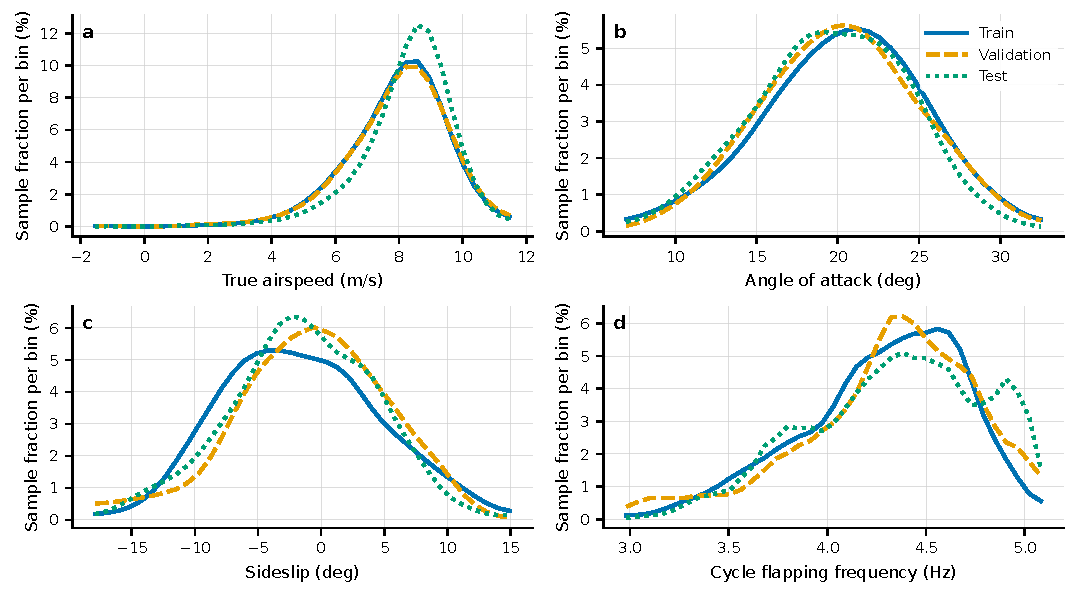
\includegraphics[width=0.88\textwidth]{figures/operating_envelope_summary.pdf}
  \caption{Operating-envelope distributions after preprocessing and whole-log splitting. Each panel shows lightly smoothed sample-fraction curves computed from common bins for true airspeed, angle of attack, sideslip, and cycle flapping frequency, using the retained samples from the training, validation, and test logs. The figure defines the flight-condition range for the log-based evaluation; it is not a closed-loop simulation or controller-performance result.}
  \label{fig:operating_envelope}
\end{figure*}

The purpose of these statistics is to define the evaluation boundary. The held-out metrics in Sec.~\ref{sec:results} measure interpolation and cross-log generalization within this retained outdoor envelope. They do not show performance for takeoff, landing, aggressive maneuvers outside the logged range, or closed-loop simulation with the learned residual model.

\subsection{Effective-Wrench Reconstruction}
\label{subsec:wrench_target}

\begin{figure}[t]
  \centering
  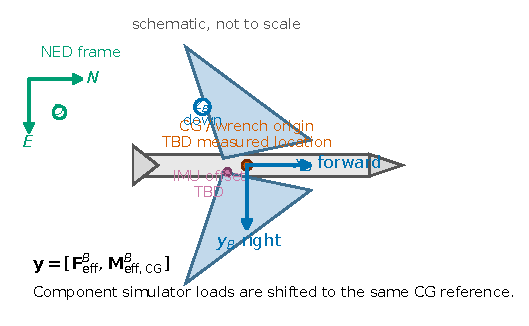
\includegraphics[width=0.98\columnwidth]{figures/wrench_reference_schematic.pdf}
  \caption{Schematic reference definition for effective-wrench reconstruction. The body frame follows forward-right-down convention and is attached to the measured center of gravity. Both the log-derived effective wrench and the simulator-prior wrench are expressed in this frame and reported about the same CG reference point. Red labels mark measured metadata values to be filled in the final draft.}
  \label{fig:wrench_reference}
\end{figure}

The target contains the three body-frame force components and the three body-frame moment components, using the reference convention summarized in Fig.~\ref{fig:wrench_reference}. We refer to this six-component vector as an effective wrench and write it as
\begin{equation}
  \mathbf{y}_t =
  \begin{bmatrix}
  f_{x,b} & f_{y,b} & f_{z,b} & m_{x,b} & m_{y,b} & m_{z,b}
  \end{bmatrix}^{\mathsf{T}},
  \label{eq:wrench_vector}
\end{equation}
where the body frame $B$ follows the forward-right-down convention, its origin is the measured center of gravity, and the navigation frame $N$ follows the north-east-down convention. The word effective is deliberate. The label is the net non-gravitational external wrench, about the measured CG, required to explain the measured rigid-body motion; it is not a direct wind-tunnel measurement of pure aerodynamic force and moment. It may include flapping-wing aerodynamics, tail and body aerodynamics, mechanism reaction effects, airdata and state-estimation errors, and outdoor disturbances.

The effective force is reconstructed from the translational dynamics. With $\mathbf{R}_{BN}$ denoting the rotation from navigation coordinates to body coordinates,
\begin{equation}
  \mathbf{F}_{\mathrm{eff}}^{B}
  =
  m\,\mathbf{R}_{BN}
  \left(
    \mathbf{a}^{N} - \mathbf{g}^{N}
  \right),
  \label{eq:force_label}
\end{equation}
where $m$ is the vehicle mass, $\mathbf{a}^{N}$ is the local-frame acceleration estimate, and $\mathbf{g}^{N}=[0,0,g]^{\mathsf{T}}$ in NED coordinates. The subtraction removes gravity before the result is expressed in body FRD coordinates, so upward lift appears as a negative $f_{z,b}$ component.

The effective moment is reconstructed from rigid-body rotational dynamics,
\begin{equation}
  \mathbf{M}_{\mathrm{eff}}^{B}
  =
  \mathbf{I}_{B}\boldsymbol{\alpha}_{B}
  +
  \boldsymbol{\omega}_{B}
  \times
  \left(
    \mathbf{I}_{B}\boldsymbol{\omega}_{B}
  \right),
  \label{eq:moment_label}
\end{equation}
where $\mathbf{I}_{B}$ is the body-frame inertia matrix about the measured CG, $\boldsymbol{\omega}_{B}$ is the body angular velocity, and $\boldsymbol{\alpha}_{B}$ is the body angular acceleration. In the current canonical pipeline, $\boldsymbol{\alpha}_{B}$ is read from the PX4 angular-velocity derivative fields; a smoothed-derivative path is also used for the sensitivity check reported later. The rigid-body metadata supplied to Eqs.~\eqref{eq:force_label}--\eqref{eq:moment_label} are \needinfo{$m=\mathrm{TBD}~\mathrm{kg}$}, \needinfo{$\mathbf{r}_{\mathrm{CG}}=\mathrm{TBD}$}, \needinfo{$\mathbf{r}_{\mathrm{IMU}/\mathrm{CG}}^{B}=\mathrm{TBD}$}, and \needinfo{$\mathbf{I}_{B,\mathrm{CG}}=\mathrm{TBD}~\mathrm{kg\,m^2}$}. These values are obtained from the three-point weighing, plumb-line CG, mechanical offset survey, and bifilar-pendulum inertia procedures described above.

The same reference point is used when comparing the log-derived wrench with the DeLaurier-style simulator prior. If the prior computes component loads at wing, tail, fuselage, or body reference points, each component is shifted to the measured CG before summation:
\begin{equation}
  \mathbf{M}_{\mathrm{sim,CG}}^{B}
  =
  \sum_j
  \left(
    \mathbf{M}_{j}^{B}
    +
    \mathbf{r}_{j/\mathrm{CG}}^{B}
    \times
    \mathbf{F}_{j}^{B}
  \right),
  \label{eq:sim_wrench_reference_shift}
\end{equation}
where $\mathbf{r}_{j/\mathrm{CG}}^{B}$ points from the measured CG to the component load reference. This alignment prevents a moment residual from being created purely by comparing two wrenches about different points. The component reference locations used for the final prior are \needinfo{TBD: wing, tail, fuselage, and body load-reference coordinates}.

\begin{table*}[t]
\caption{Main error sources in log-based effective-wrench labels and the associated checks used to bound them. Red entries mark numerical values to be filled with the final measurement and sensitivity results.}
\label{tab:wrench_error_sources}
\centering
\resizebox{\textwidth}{!}{%
\begin{tabular}{@{}p{0.18\textwidth}p{0.45\textwidth}p{0.28\textwidth}@{}}
\toprule
Source & How it enters the reconstructed label & Measurement or sensitivity record \\
\midrule
Acceleration noise & Directly changes $\mathbf{F}_{\mathrm{eff}}^{B}$ after gravity compensation. & Force-label smoothing sensitivity \needinfo{TBD: filter/window and force RMSE or label variation}. \\
Attitude error & Rotates both gravity-compensated acceleration and derived air-relative quantities. & Estimator quality and attitude innovation summary \needinfo{TBD}. \\
Rate and acceleration differentiation & Affects $\boldsymbol{\alpha}_{B}$ and therefore the moment label. & Angular-acceleration smoothing sensitivity \needinfo{TBD: moment-label variation and selected derivative path}. \\
Time alignment & Misaligns state, actuation, airdata, and phase at wingbeat time scales. & Topic age limits and phase-alignment check \needinfo{TBD: maximum age / phase delay tolerance}. \\
Mass, inertia, and CG uncertainty & Scales force and moment and changes the moment reference assumptions. & Three-point weighing, plumb-line CG, and bifilar-pendulum inertia; perturbation sensitivity \needinfo{TBD: mass, CG offset, inertia ranges}. \\
Reference-point mismatch & Creates artificial moment residuals when component loads and reconstructed moments are not expressed about the same point. & All prior component loads shifted to measured CG using Eq.~\eqref{eq:sim_wrench_reference_shift}; component coordinates \needinfo{TBD}. \\
Unmodeled mechanism reaction & Appears in the effective wrench but is not separable from aerodynamic load. & Treated as part of effective wrench; mechanism-state diagnostic \needinfo{TBD if included}. \\
Airdata and wind estimation & Affects model inputs and flight-condition interpretation. & Logged airdata and wind freshness plus campaign weather record \needinfo{TBD}. \\
Sensor freshness & Low-rate airdata, wind, GPS, and status topics are held with age masks. & Freshness thresholds and retained-valid fraction \needinfo{TBD}. \\
\bottomrule
\end{tabular}%
}
\end{table*}

These errors enter the supervised target itself. Consequently, the residual analyzed later should not be interpreted as one unique physical mechanism. It is a simulator-to-flight effective-wrench discrepancy under the sensing, metadata, and reconstruction assumptions above.

\subsection{Preprocessing, Model Inputs, and Whole-Log Split}
\label{subsec:canonical_samples}

Raw ULog topics are converted to a canonical $100~\mathrm{Hz}$ grid before model training. The preprocessing code constructs a uniform timeline from the core high-rate topics and then applies topic-specific resampling rules. Actuator motor and servo commands are averaged within each $10~\mathrm{ms}$ bin. Continuous states such as local position, velocity, acceleration, attitude quaternion components, angular velocity, and angular acceleration are linearly resampled on the grid, with quaternion normalization performed during downstream derived-feature construction. Low-rate airdata, wind, GPS, status, and allocator-status topics are held with zero-order hold and freshness masks. These freshness flags keep stale low-rate values identifiable instead of silently treating them as synchronous high-rate measurements.

Wingbeat phase is handled separately because it is central to the residual structure. The pipeline first reconstructs encoder and drive phase from encoder counts and metadata. If a fresh \texttt{wing\_phase} topic is present, as in the present paper split, that Hall-indexed phase becomes the raw phase source. The pipeline then annotates active flapping cycles, removes incomplete edge cycles, and maps each valid cycle to a corrected $[0,2\pi]$ phase coordinate. The final retained rows therefore satisfy \texttt{flap\_active}, \texttt{cycle\_valid}, and \texttt{label\_valid}. This filtering is why the sample counts in Table~\ref{tab:log_split_envelope} are lower than the raw ULog row counts.

The model inputs are organized into four groups. The state group contains attitude-derived quantities, body angular velocity, local and body-frame velocities, gravity direction, and air-relative velocity quantities such as angle of attack and sideslip. The actuation group contains the flapping motor command and the three tail-surface commands, including elevator-like and aileron-like combinations of the horizontal-tail pair. The flapping group contains corrected phase, phase sine and cosine, wing-stroke angle, flapping frequency, and cycle-level flapping frequency. The airdata group contains measured airspeed, air density, dynamic pressure, and wind estimates. These groups are used both for memoryless baselines and for causal temporal models, where phase, actuation, and airdata histories are allowed while current-state quantities are provided only at the prediction time.

The input design enforces a causal reconstruction boundary. Translational acceleration, angular acceleration, and past wrench targets are not provided as neural-model inputs in the paper feature set; acceleration is used only to reconstruct Eq.~\eqref{eq:force_label}, and angular acceleration is used only in Eq.~\eqref{eq:moment_label}. This prevents the network from learning the label by reading the same acceleration channels used to define it.

Finally, the dataset is split at the whole-log level to avoid temporal leakage. Splitting one flight log across training and testing would place nearby samples with similar phase, actuator history, airdata, wind condition, estimator history, and airframe condition in different sets. The current high-quality paper split therefore contains 29 logs: 20 training logs, 5 validation logs, and 4 test logs. The corresponding sample counts are 308702 training samples, 79587 validation samples, and 60671 test samples.

% !TeX root = ../main.tex
\section{Theory-Guided Neural Residual Model}
\label{sec:method}

\subsection{Physics-Based Aerodynamic Model and Calibration}
\label{subsec:delaurier_calibration}

A physics-based aerodynamic model based on DeLaurier's flapping-wing formulation~\cite{delaurier1993} provides the structured part of the wrench prediction. The model is implemented in IsaacLab and produces the same six-component body-frame force and moment vector as the effective-wrench target in Eq.~\eqref{eq:wrench_vector}. It uses the wing motion, local airdata, body rates, and tail and fuselage terms required by the aerodynamic calculation.

The model is useful because it maps vehicle geometry, wing motion, and flight condition to a physically organized wrench estimate. The formulation relies on strip-theory and quasi-steady assumptions, approximate geometry and aerodynamic parameters, and simplified treatments of wing flexibility, unsteady loading, and tail/body aerodynamics. These approximations make the model incomplete for outdoor free flight. We therefore use the calibrated aerodynamic model as the baseline physical prediction and train a neural residual estimator for the remaining discrepancy.

Before residual training, the aerodynamic model is calibrated using training logs only. The calibration is low-dimensional and bounded: it adjusts only the parameters listed below, while leaving the aerodynamic structure fixed. The optimized parameter vector is
\begin{equation}
\boldsymbol{\psi}
=
(s_N,\;s_C,\;\theta_w,\;\eta_{\max},\;e_i,\;C_{D,A},\;s_T,\;\Delta t_{\phi}).
\label{eq:prior_params}
\end{equation}
Here $s_N$, $s_C$, and $s_T$ scale wing normal force, wing chordwise force, and tail lift; $\theta_w$ and $\eta_{\max}$ set wing incidence and twist; $e_i$ and $C_{D,A}$ parameterize induced drag and fuselage drag; and $\Delta t_{\phi}$ is the phase delay. After calibration, $\boldsymbol{\psi}$ is fixed and the calibrated model provides the baseline prediction used to define the residual target.

The calibration objective minimizes a weighted discrepancy between the log-derived effective wrench and the physics-based model. With
\begin{equation}
  \mathbf{d}_t(\boldsymbol{\psi})
  =
  \mathbf{W}
  \left[
    \mathbf{y}_t-\mathbf{y}^{D}_t(\boldsymbol{\psi})
  \right],
  \label{eq:prior_calibration_residual}
\end{equation}
the calibrated parameters are obtained from
\begin{equation}
  \begin{aligned}
  \boldsymbol{\psi}^{\star}
  &=
  \arg\min_{\boldsymbol{\psi}\in\Psi}
  \mathcal{J}(\boldsymbol{\psi}),\\
  \mathcal{J}(\boldsymbol{\psi})
  &=
  \frac{1}{|\mathcal{D}_{\mathrm{train}}|}
  \sum_{t\in\mathcal{D}_{\mathrm{train}}}
  \rho_{\delta}\!\left(\mathbf{d}_t(\boldsymbol{\psi})\right)
  +
  \lambda\|\boldsymbol{\psi}-\boldsymbol{\psi}_0\|_2^2 .
  \end{aligned}
  \label{eq:prior_calibration_objective}
\end{equation}
where $\Psi$ is the bounded physically plausible search region, $\mathbf{W}$ balances the six wrench channels, $\rho_{\delta}(\cdot)$ is an elementwise Huber loss, and the weak regularization term penalizes large deviations from the nominal parameters. This objective can remove systematic scale, offset, efficiency, and phase mismatch, but it does not allow the calibrated model to fit arbitrary sample-level errors.

\subsection{Channel-Aware Residual Learning and Causal Transformer}
\label{subsec:residual_learning}

The calibrated aerodynamic model is most useful for the force channels, where the
dominant wing and tail loads are represented explicitly. For the moment channels,
the same model is more sensitive to center-of-gravity location, moment arms, tail
modeling, and small label variance. The final hybrid model therefore uses a
channel-aware output definition. Let
$\mathcal{F}=\{f_{x,b},f_{y,b},f_{z,b}\}$ and
$\mathcal{M}=\{m_{x,b},m_{y,b},m_{z,b}\}$. The force prediction is
\begin{equation}
  \hat{\mathbf{y}}_{t,\mathcal{F}}
  =
  \mathbf{y}^{D}_{t,\mathcal{F}}(\mathbf{z}_t;\boldsymbol{\psi}^{\star})
  +
  \hat{\mathbf{r}}_{\theta,t,\mathcal{F}},
  \label{eq:hybrid_force}
\end{equation}
and the moment prediction is
\begin{equation}
  \hat{\mathbf{y}}_{t,\mathcal{M}}
  =
  \hat{\mathbf{m}}_{\theta,t}.
  \label{eq:hybrid_moment}
\end{equation}
Here $\mathbf{z}_t$ denotes the aerodynamic-model inputs at time $t$,
$\mathbf{y}^{D}_{t,\mathcal{F}}$ is the calibrated force prediction,
$\hat{\mathbf{r}}_{\theta,t,\mathcal{F}}$ is the neural force residual, and
$\hat{\mathbf{m}}_{\theta,t}$ is the direct neural moment prediction. The force
residual target is
\begin{equation}
  \mathbf{r}_{t,\mathcal{F}}
  =
  \mathbf{y}_{t,\mathcal{F}}
  -
  \mathbf{y}^{D}_{t,\mathcal{F}} .
  \label{eq:force_residual_target}
\end{equation}

The force residual is a combined discrepancy between the calibrated aerodynamic
model and the real-flight effective wrench. It can arise from wing flexibility,
unsteady loading, remaining parameter mismatch, actuator timing, tail/body
aerodynamic mismatch, outdoor disturbances, and wrench-label reconstruction
error. The neural model therefore learns a correction to the calibrated force
prediction, while the moment head learns the moment components directly.
Further analysis identifies which parts of the force correction are repeatable
with phase, frequency, or flight condition.

A memoryless MLP is the simplest neural correction, but flapping-wing loads depend strongly on recent wing motion, actuator response, and vehicle motion. We therefore use causal temporal models that predict the correction outputs at time $t$ from current and historical onboard-measurable variables. Among the tested recurrent, convolutional, and attention-based backbones, the Transformer gave the best validation accuracy and is used as the main estimator:
\begin{equation}
  \left[
  \hat{\mathbf{r}}_{\theta,t,\mathcal{F}},
  \hat{\mathbf{m}}_{\theta,t}
  \right]
  =
  f_{\theta}
  \left(
    \mathbf{s}_{t-H+1:t},
    \mathbf{c}_{t}
  \right),
  \label{eq:residual_causal_model}
\end{equation}
where $\mathbf{s}_{t-H+1:t}$ is a causal history window and $\mathbf{c}_t$ contains current-time features. Consistent with the input organization in Sec.~\ref{subsec:canonical_samples}, the history contains phase, flapping, actuation, and airdata variables, while the current features contain state and air-relative quantities. Acceleration channels and past wrench targets are excluded, so the estimator uses only variables that are measurable onboard before the target wrench is reconstructed.

\subsection{Residual Signals for Analysis}
\label{subsec:residual_structure_methods}

For the force channels, the residual formulation also defines the quantities used
for post-training analysis:
\begin{equation}
  \begin{aligned}
  \mathbf{r}_{t,\mathcal{F}}
  &=
  \mathbf{y}_{t,\mathcal{F}} - \mathbf{y}^{D}_{t,\mathcal{F}},\\
  \mathbf{e}_{t,\mathcal{F}}
  &=
  \mathbf{y}_{t,\mathcal{F}}
  - \mathbf{y}^{D}_{t,\mathcal{F}}
  - \hat{\mathbf{r}}_{\theta,t,\mathcal{F}} .
  \end{aligned}
  \label{eq:residual_triplet}
\end{equation}
Here $\mathbf{r}_{t,\mathcal{F}}$ is the force residual left by the calibrated
aerodynamic model, $\hat{\mathbf{r}}_{\theta,t,\mathcal{F}}$ is the neural
force-residual prediction, and $\mathbf{e}_{t,\mathcal{F}}$ is the remaining force residual
after correction. These three signals are later compared across wingbeat phase,
flight condition, and frequency band to determine whether the force residual
contains repeatable structure.

% !TeX root = ../main.tex
\section{Evaluation Protocol}
\label{sec:evaluation}

\subsection{Compared Models}
\label{subsec:compared_models}

We compare four models from the measured-mass-properties branch. The calibrated aerodynamic model is the DeLaurier-style prior after train-only affine force alignment of the exported prior predictions. The first correction model applies a force-only structured correction and leaves the prior moment channels unchanged; it tests whether real-flight force residuals can be reduced without introducing a moment model. The deployable correction extends this model with simulator-available rates, airdata, phase, and control features for both force and effective-moment prediction. The phase-structured correction uses the same deployable feature boundary and adds explicit wingbeat-phase harmonic and interaction terms, giving the final correction used for residual-structure analysis.

Together, these models separate the effects of affine prior alignment, structured force correction, deployable input constraints, and channel-specific output semantics. The comparison is intentionally log-conditioned: every model is evaluated against the reconstructed effective-wrench labels on held-out logs, not by replaying the vehicle trajectory in closed-loop simulation.

\subsection{Train/Validation/Test and Cross-Validation}
\label{subsec:split_protocol}

The primary experiment uses the fixed whole-log split described in Sec.~\ref{subsec:canonical_samples}. Prior alignment and correction fitting use training logs only. Model families and ridge regularization values are selected using validation logs, and the selected models are evaluated once on held-out test logs. Normalization statistics, affine prior-alignment parameters, feature fill values, and model-selection decisions are not fitted on test logs.

In the measured-mass-properties rerun, the fixed paper split is the primary evidence. The test split contains four complete logs from four flight dates, so per-log metrics are also reported to show how much the fixed-split result varies across held-out log composition. A full date-stratified cross-validation rerun with the measured-mass-properties branch is left as an optional robustness check before final submission.

\subsection{Replay Diagnostics}
\label{subsec:replay_diagnostics}

Replay is used only as a diagnostic for label construction, not as a primary validation metric. Outdoor open-loop replay compounds state-estimation noise, smoothing choices, time alignment, wind and disturbance terms, and controller-response mismatch. A corrected instantaneous effective-wrench map can be useful for simulation even when strict open-loop replay of the logged raw trajectory is not possible.

We therefore run alpha-only replay checks to verify the rotational label pathway. Moment-inferred angular acceleration is compared against the smoothed angular acceleration used for label construction, and the smoothed acceleration is integrated over short windows to quantify how closely it returns to the raw logged gyro. These checks diagnose the smoothing and label definitions; they do not validate closed-loop simulator behavior.

\subsection{Metrics}
\label{subsec:metrics}

The primary metrics are per-target root-mean-square error (RMSE) and mean absolute error (MAE):
\begin{equation}
  \mathrm{RMSE}_{j}
  =
  \sqrt{
    \frac{1}{N}
    \sum_{n=1}^{N}
    \left(
      \hat{y}_{n,j} - y_{n,j}
    \right)^2
  },
  \label{eq:rmse}
\end{equation}
\begin{equation}
  \mathrm{MAE}_{j}
  =
  \frac{1}{N}
  \sum_{n=1}^{N}
  \left|
    \hat{y}_{n,j} - y_{n,j}
  \right|.
  \label{eq:mae}
\end{equation}
Aggregate RMSE and MAE are reported as compact summaries, but per-target values are the main evidence because the six wrench channels have different units, amplitudes, excitation levels, and label quality.

To give the absolute errors a scale reference, we also report the held-out
standard deviation $\sigma_{y,j}$ of each target channel and the normalized
error $\mathrm{RMSE}_j/\sigma_{y,j}$. We report $R^2$ as a secondary metric.
Because the six channels have different scales and excitation levels, $R^2$ is
interpreted together with RMSE, MAE, and $\mathrm{RMSE}/\sigma_y$. This is
especially important for moment channels, where the label variance is much
smaller than in the force channels.

% !TeX root = ../main.tex
\section{Results and Discussion}
\label{sec:results}

\subsection{Calibration and Residual Prediction Performance}
\label{subsec:prediction_performance}

Physical calibration makes the aerodynamic model more consistent with the real
vehicle. On the held-out test split, force RMSE decreases from $6.64$ to
$5.42~\mathrm{N}$ for $f_{x,b}$, from $6.11$ to $3.52~\mathrm{N}$ for
$f_{y,b}$, and from $18.43$ to $13.10~\mathrm{N}$ for $f_{z,b}$. Moment RMSE
also decreases, from $0.152$ to $0.071~\mathrm{N\,m}$ for $m_{x,b}$, from
$1.285$ to $0.602~\mathrm{N\,m}$ for $m_{y,b}$, and from $0.211$ to
$0.102~\mathrm{N\,m}$ for $m_{z,b}$. This confirms that the calibrated
aerodynamic model is meaningful, while also showing that a large real-flight
residual remains.

Table~\ref{tab:residual_overall_results} compares the calibrated aerodynamic
model, direct black-box prediction, and neural corrections. The calibrated model
has an overall RMSE of $5.965$ on the sequence-aligned held-out rows. Adding a
residual MLP reduces RMSE to $2.481$, showing that instantaneous variables
explain a substantial part of the residual. The channel-aware hybrid Transformer
further reduces RMSE to $0.870$ and MAE to $0.443$, while using residual
correction for forces and direct prediction for moments. The direct Transformer
reaches a similar RMSE of $0.888$. These results show that the hybrid
formulation keeps black-box-level predictive accuracy while retaining an explicit
calibrated aerodynamic model for the force residual analysis below.

\begin{table}[t]
\centering
\caption{Held-out test comparison. Values are computed on each model's aligned test rows.}
\label{tab:residual_overall_results}
\resizebox{\columnwidth}{!}{%
\begin{tabular}{@{}lccc@{}}
\toprule
Method & Rows & RMSE & MAE \\
\midrule
Calibrated aerodynamic model & 58639 & 5.965 & 2.961 \\
Direct Transformer & 58639 & 0.888 & 0.455 \\
Calibrated model + residual MLP & 60671 & 2.481 & 1.286 \\
Channel-aware hybrid Transformer & 58639 & \textbf{0.870} & \textbf{0.443} \\
\bottomrule
\end{tabular}%
}
\end{table}

Target-wise results in Table~\ref{tab:residual_target_results} show that the
largest absolute improvements occur in the main force channels. For $f_{x,b}$,
RMSE decreases from $5.416$ to $0.780~\mathrm{N}$; for $f_{z,b}$, it decreases
from $13.091$ to $1.581~\mathrm{N}$. The side-force channel remains the hardest
force component, with $\mathrm{RMSE}/\sigma_y=0.828$, but still improves from
$3.521$ to $1.196~\mathrm{N}$. For the
moment channels, direct neural prediction is more appropriate than residual
correction to the calibrated moment output. The channel-aware model reduces
moment RMSE to $0.0021$, $0.0012$, and $0.00033~\mathrm{N\,m}$ for
$m_{x,b}$, $m_{y,b}$, and $m_{z,b}$, respectively, with positive $R^2$ in all
three channels.

\begin{table}[t]
\centering
\caption{Target-wise held-out test metrics for the calibrated aerodynamic model and channel-aware hybrid Transformer. $\sigma_y$ is the standard deviation of the held-out target channel. For force channels, the hybrid model uses calibrated-model residual correction; for moment channels, it uses direct prediction.}
\label{tab:residual_target_results}
\resizebox{\columnwidth}{!}{%
\begin{tabular}{@{}lcccccc@{}}
\toprule
Target & $\sigma_y$ & Model RMSE & Hybrid RMSE & RMSE/$\sigma_y$ & Hybrid MAE & Hybrid $R^2$ \\
\midrule
$f_{x,b}$ & 4.826 & 5.416 & 0.780 & 0.162 & 0.592 & 0.974 \\
$f_{y,b}$ & 1.445 & 3.521 & 1.196 & 0.828 & 0.866 & 0.315 \\
$f_{z,b}$ & 9.294 & 13.091 & 1.581 & 0.170 & 1.197 & 0.971 \\
$m_{x,b}$ & 0.00332 & 0.0716 & 0.00210 & 0.633 & 0.00152 & 0.599 \\
$m_{y,b}$ & 0.00432 & 0.5997 & 0.00123 & 0.285 & 0.00094 & 0.919 \\
$m_{z,b}$ & 0.000510 & 0.1018 & 0.000327 & 0.642 & 0.000250 & 0.588 \\
\bottomrule
\end{tabular}%
}
\end{table}

\subsection{Cross-Log Generalization}
\label{subsec:kfold_results}

The five-fold whole-log evaluation checks whether the channel-aware hybrid
model is stable across different held-out log compositions. Across folds, the
calibrated aerodynamic model has overall RMSE $5.883\pm0.040$ and MAE
$2.918\pm0.016$, while the hybrid model reduces these values to
$0.865\pm0.027$ and $0.443\pm0.014$. The force-channel RMSE is
$1.223\pm0.038~\mathrm{N}$, and the moment-channel RMSE is
$0.00131\pm0.00007~\mathrm{N\,m}$. The low fold-to-fold variability shows that
the calibrated model leaves a stable force residual and that the causal hybrid
model transfers across held-out log composition.

\begin{table}[t]
\centering
\caption{Date-stratified five-fold whole-log evaluation for the channel-aware hybrid Transformer. Values are mean $\pm$ standard deviation over folds.}
\label{tab:kfold_results}
\resizebox{\columnwidth}{!}{%
\begin{tabular}{@{}lcccc@{}}
\toprule
Target & Model RMSE & Hybrid RMSE & Hybrid MAE & Hybrid $R^2$ \\
\midrule
Overall & $5.883{\pm}0.040$ & $\mathbf{0.865{\pm}0.027}$ & $\mathbf{0.443{\pm}0.014}$ & -- \\
$f_{x,b}$ & $5.379{\pm}0.091$ & $0.811{\pm}0.043$ & $0.617{\pm}0.031$ & $0.971{\pm}0.003$ \\
$f_{y,b}$ & $3.443{\pm}0.062$ & $1.049{\pm}0.041$ & $0.784{\pm}0.029$ & $0.406{\pm}0.043$ \\
$f_{z,b}$ & $12.904{\pm}0.099$ & $1.652{\pm}0.055$ & $1.255{\pm}0.043$ & $0.967{\pm}0.002$ \\
$m_{x,b}$ & $0.0658{\pm}0.0029$ & $0.00191{\pm}0.00013$ & $0.00142{\pm}0.00009$ & $0.626{\pm}0.084$ \\
$m_{y,b}$ & $0.5907{\pm}0.0233$ & $0.00118{\pm}0.00004$ & $0.00090{\pm}0.00003$ & $0.924{\pm}0.006$ \\
$m_{z,b}$ & $0.1020{\pm}0.0022$ & $0.000318{\pm}0.000019$ & $0.000242{\pm}0.000014$ & $0.546{\pm}0.054$ \\
\bottomrule
\end{tabular}%
}
\end{table}

\subsection{Residual Structure Analysis}
\label{subsec:residual_structure_results}

The residual diagnostics answer whether the calibrated force-model mismatch is
random or structured. Fig.~\ref{fig:residual_structure} summarizes the three
most informative views: wingbeat-phase medians, condition-binned residual RMSE,
and frequency-band energy. In each case, the comparison is between the force
residual $\mathbf{r}_{t,\mathcal{F}}$, the neural prediction
$\hat{\mathbf{r}}_{\theta,t,\mathcal{F}}$, and the remaining force residual
$\mathbf{e}_{t,\mathcal{F}}$ after correction.

\begin{figure*}[t]
  \centering
  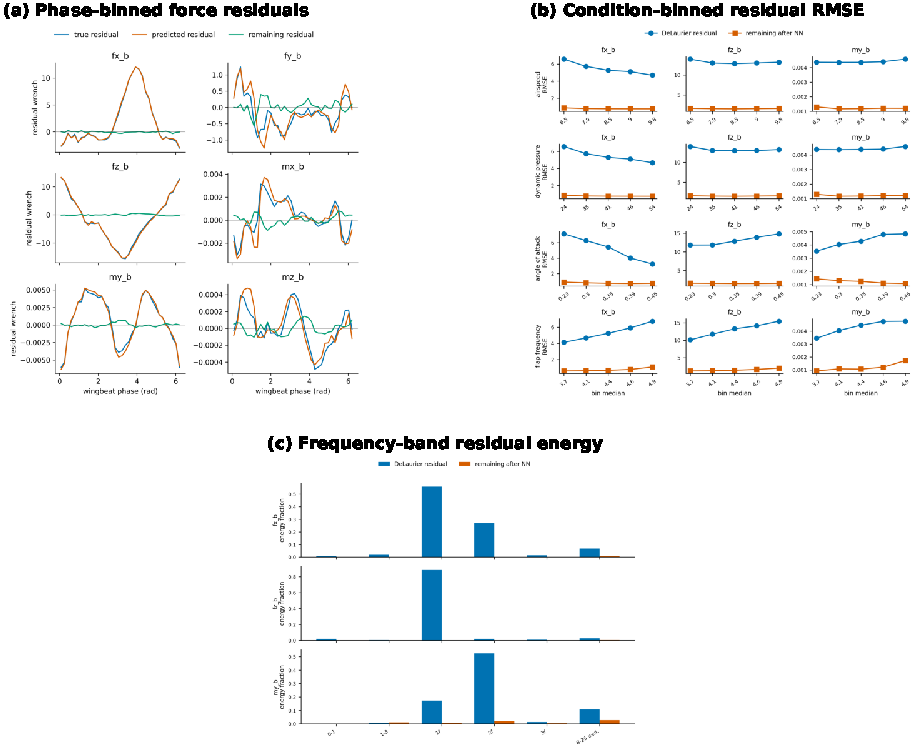
\includegraphics[width=\textwidth]{figures/residual_structure_summary.pdf}
  \caption{Force residual structure before and after neural correction. Panel (a) compares phase-binned median residuals. Panel (b) shows condition-binned residual RMSE. Panel (c) shows demeaned residual energy by frequency band; the shaded bars are remaining residual energy normalized by the original calibrated-model residual energy.}
  \label{fig:residual_structure}
\end{figure*}

\textit{Phase structure.} The main force-channel residuals contain repeatable wingbeat-phase waveforms, which indicates that the calibrated aerodynamic model leaves a cycle-synchronous mismatch rather than only random log noise. For $f_{x,b}$, phase-bin medians explain $0.817$ of the true residual variance and have a peak-to-peak amplitude of $15.10~\mathrm{N}$. For $f_{z,b}$, the corresponding phase $R^2$ is $0.509$ and the peak-to-peak amplitude is $28.79~\mathrm{N}$. The neural prediction follows these median waveforms closely, including the large positive $f_{x,b}$ residual during the latter half of the wingbeat and the sign-changing $f_{z,b}$ waveform over the cycle. After correction, the remaining phase peak-to-peak amplitudes fall to $0.56~\mathrm{N}$ and $0.98~\mathrm{N}$, respectively. This reduction is important because the model removes a repeatable intra-wingbeat component that the quasi-steady aerodynamic calculation does not capture.

\textit{Flight-condition dependence.} The force residual also varies across operating conditions, so the mismatch is not described completely by phase alone. The strongest dependence appears in $f_{x,b}$ versus angle of attack: residual RMSE changes by a factor of $2.21$ across bins, with the worst bin reaching $7.145~\mathrm{N}$. For $f_{z,b}$, the largest residual occurs at high angle of attack, reaching $14.809~\mathrm{N}$. Fig.~\ref{fig:residual_structure}(c) shows that the two force components have different trends with angle of attack: the calibrated model becomes less accurate in $f_{z,b}$ as angle of attack increases, while $f_{x,b}$ has larger residuals at the lower-angle bins in this flight envelope. Flapping frequency is also important: the highest-frequency bin reaches $6.735~\mathrm{N}$ in $f_{x,b}$ and $15.466~\mathrm{N}$ in $f_{z,b}$. The channel-aware hybrid model reduces the worst-bin errors to $0.896~\mathrm{N}$ and $2.059~\mathrm{N}$, respectively, but the remaining errors are not perfectly uniform across bins. This suggests that the learned correction is effective inside the observed envelope while still reflecting where the real-flight data provide more difficult or less repeated conditions.

\textit{Frequency-domain structure.} After subtracting segment means, most residual energy is organized around the flapping cycle. In $f_{x,b}$, $55.9\%$ of the residual energy is at the wingbeat fundamental and $26.9\%$ at the second harmonic. In $f_{z,b}$, the fundamental carries $88.4\%$ of the demeaned residual energy. These numbers are consistent with the phase-binned result: the force-model mismatch is dominated by repeatable periodic components, not by an arbitrary offset. The hybrid model removes nearly all of these components. In the dominant wingbeat-fundamental band, the remaining energy is only $0.27\%$ of the original band energy for $f_{x,b}$ and $0.13\%$ for $f_{z,b}$. Broadband high-frequency content is reduced less strongly, consistent with that band containing more sensor noise, effective-wrench reconstruction error, or nonrepeatable outdoor disturbance.

Together, these analyses show that the neural force residual is not merely lowering aggregate RMSE. It removes a structured discrepancy left by the calibrated aerodynamic model: a wingbeat-synchronous component, a flight-condition-dependent component, and a frequency-localized component. The remaining residual is therefore a more plausible mixture of unmodeled stochastic disturbance, label reconstruction noise, and operating points where the available flight logs provide weaker excitation.

\subsection{Interpretation and Limitations}
\label{subsec:interpretation_limitations}

The calibrated aerodynamic model provides a physically organized baseline. The
key result is that the force residual left by this baseline is stable and
interpretable. In the main force channels, the residual model mainly learns
wingbeat-synchronous correction. In the moment channels, the final model uses
direct neural prediction because the calibrated moment output is dominated by
large bias relative to the small measured moment range. The side-force channel
remains the most difficult force component, likely because of weaker lateral
excitation, wind disturbance, sideslip-estimation sensitivity, and label noise.

The residual should not be assigned to a single physical cause. It may reflect wing flexibility, unsteady loading, phase delay, actuator timing, tail/body coupling, airframe-specific parameters, or effective-wrench label reconstruction. The value of the residual analysis is narrower but still useful: it shows where the simulator prior is systematically mismatched and which parts of that mismatch can be learned from onboard measurements.

The present evaluation is log-based. It shows that the hybrid model predicts held-out effective wrench and removes structured force residual content, but it is not yet a closed-loop simulation validation. The next step is to embed the hybrid model in IsaacLab and evaluate short-horizon trajectory replay and controller performance. The dataset is also from one platform and a limited outdoor envelope, so future data should deliberately cover broader angle-of-attack, flapping-frequency, sideslip, and wind conditions, ideally with uncertainty estimates for out-of-envelope use.

% !TeX root = ../main.tex
\section{Conclusion}
\label{sec:conclusion}

This paper presented a real-flight effective-wrench correction pipeline for a bird-scale flapping-wing vehicle. A DeLaurier-style aerodynamic model was used as a low-dimensional simulator prior, aligned with training logs through a force-channel affine wrapper, and then compared with six-component effective-wrench labels reconstructed from outdoor PX4 flight logs using measured mass, center-of-gravity, and inertia properties.

The main finding is that an affine-aligned flapping-wing aerodynamic prior leaves a structured real-flight force residual, and this residual can be reduced with a deployable phase- and condition-dependent correction. On held-out logs, the phase-structured correction reduced force-channel RMSE by $68.3\%$ for $f_{x,b}$, $15.0\%$ for $f_{y,b}$, and $69.8\%$ for $f_{z,b}$ relative to the affine-aligned prior. Effective moment channels were also predicted, with the strongest result in $m_{y,b}$, but the moment results remain more sensitive to inertia, reference-point consistency, and angular-acceleration smoothing.

Residual analysis showed that the prior mismatch is not arbitrary. The main force-channel residuals contain wingbeat-phase, frequency, and flight-condition structure, and the structured correction removes much of this repeatable component on held-out logs. This supports real-flight data as a practical way to build a log-conditioned correction around a low-dimensional flapping-wing simulator prior without replacing the prior with an unrestricted black-box model.

The corrected map is a prerequisite step toward simulator embedding, not a completed closed-loop simulation validation. Replay was used here only as a diagnostic because outdoor replay compounds estimator noise, smoothing choices, time alignment, wind disturbance, and controller-response mismatch. Future work will embed the correction into IsaacLab with explicit disturbance and uncertainty handling, evaluate controller-in-the-loop behavior, and collect broader flight data over angle-of-attack, flapping-frequency, sideslip, wind, and maneuver conditions.


\acknowledgements
TODO: Add funding, sponsor, clearance, and AI-use disclosure statements as appropriate before submission.

\bibliographystyle{IEEEtran}
\bibliography{bib/refs,bib/flapping_nn_related}

\thebiography

\begin{biography}{TODO Author Name}
TODO: Add a short biography for each author. Replace this placeholder once the final author list is known.
\end{biography}

\end{document}
